\section{Corrientes relacionadas}

Los juegos serios son el solapamiento de tres corrientes, los videojuegos, las
técnicas de enseñanza y la simulación educativa\cite{education:games}, tal y
como se observa en la figura~\ref{fig:corrientes_relacionadas}. 

\begin{figure}[ht]
\centering
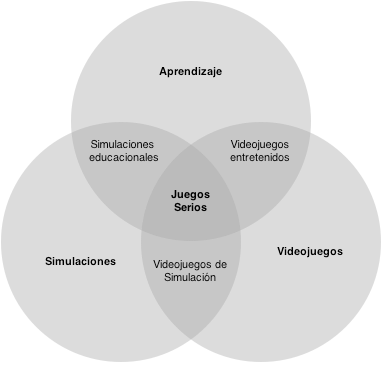
\includegraphics[scale=0.7]{juegos_serios/corrientes_paralelas.png}
\caption{Ubicación de los juegos serios entre los videojuegos, la simulación y
    la educación}
\label{fig:corrientes_relacionadas}
\end{figure}

Cuando se utilizan aspectos de videojuegos con simulaciones, se obtienen videojuegos,
cuyo objetivo es entretener mientras son similares a la realidad, dentro de esta
categoría podemos encontrar juegos como \emph{Gran Turismo}; sí mezclamos
factores relacionados al aprendizaje y a las simulaciones se obtienen
simulaciones sin interacción con el usuario que buscan mostrar o enseñar como se
comportan distintos fenómenos físicos, sociales, etc.

Los \emph{Edutainment} pueden ser vistos como los predecesores de los juegos
serios, los mismos son descritos en~\ref{sec:edutainment}.

\subsection{Simulaciones educativas}


La simulación se define como el proceso de diseñar un modelo de un sistema real
y, llevar a cabo experimentos con este modelo, con el fin o bien de entender el
comportamiento del sistema o de la evaluación de distintas estrategias para la
operación del sistema\cite{ingalls2008introduction}. 

Aunque un juego serio y una simulación pueden parecer muy similares, se
diferencian en que, si bien muchos videojuegos incluyen una simulación, una
simulación no utiliza características típicas de los videojuegos como la fantasía,
puntuación, etc\cite{sg:aoverview}.

La simulación en el ámbito de la educación evolucionó desde simples motores de
reglas hasta complejos entornos. La simulación demostró ser una herramienta muy
útil en el ámbito laboral\cite{mariluz:seiousgames}, pues enseña al usuario a
encarar situaciones muy difíciles de representar en entornos completamente
controlados y provee mecanismos para comprobar la efectividad de la herramienta. 

Actualmente la simulación se utiliza más en el ámbito empresarial pues las
empresas son las más necesitadas de innovar en el ámbito de la enseñanza. Un
ejemplo de esta necesidad se da, por ejemplo, en el entrenamiento de nuevos
vendedores, es muy difícil enseñar a un vendedor como debe vender los productos
con un pizarrón y/o una presentación, en cambio la simulación permite que el
mismo pueda probar cosas nuevas y experiencias de sus compañeros (o instructor),
convirtiendo así el aprendizaje en colectivo\cite{mariluz:seiousgames}.

Existen dos tipos de simulaciones, en primer lugar están las experimentales que
ponen al estudiante en el lugar de un profesional y requieren que el mismo tome
decisiones para alcanzar los objetivos y en segundo lugar están las simbólicas
que buscan que el estudiante deduzca eventos, principios y mejores
prácticas\cite{charsky:2010}. 


\subsection{Diferencia entre juegos serios, simulaciones y los Edutainment}

Estos tres entornos virtuales altamente interactivos, poseen posibilidades y
fines distintos, pueden parecer similares pero poseen las siguientes
diferencias\cite{education:games}:

\begin{itemize}
\item \textbf{Simulaciones educativas}: utilizan escenarios rigurosamente
    estructurados con un conjunto altamente refinado de normas, retos y
    estrategias que son cuidadosamente diseñados para desarrollar las
    competencias específicas que se pueden transferir directamente al mundo
    real.
\item \textbf{Videojuegos:} son actividades atractivas y divertidas que
    habitualmente se utilizan exclusivamente para el entrenamiento pero también
    permiten una exposición con un conjunto determinado de herramientas,
    argumentos o ideas. Todas las partidas se juegan en un mundo estructurado
    por normas específicas, mecanismos de retroalimentación, y las herramientas
    necesarias, aunque no están tan definidas como en las simulaciones.
\item \textbf{Edutainment:} son aplicaciones educativas cuyo principal propósito
    es el de entretener, y el aprendizajes es un añadido. Los
    \emph{edutainment}, se centran en la motivación externa.
\end{itemize}
